%!TEX root = thesis.tex
\chapter{Interconnect}
\label{sec:interconnect}
ReconOS provides exceptional transparency regarding the implementation and
execution mode of a thread over the hardware/software boundary. However, the
delegate mechanism introduces an overhead for communication between threads
running in hardware. While for computational intensive tasks with low
communication demand the overhead is acceptable, for low-latency applications
with real-time aspects it breaks the overall performance significantly.
Especially for \acp{PAC}, utilizing the \ac{FPGA} for low-latency and
performance critical parts of the controller, a fast communication is crucial.

This chapter addresses the topic of communication overhead and investigates
ways to speedup the on-chip communication without loosing transparency or
burden the developer with additional tasks. Starting with a short description
of the current system, different approaches from the literature are discussed
and compared. The final architecture is then presented and evaluated.

\section{Limitations of Delegate Mechanism}
While the basic concepts of the delegate mechanism were already discussed in
the background section, a detailed knowledge of its implementation and
performance limitations is required. Consider figure \ref{fig:delegate},
showing a detailed view of the delegate implementation, consisting out of
communication interfaces, interrupt lines and drivers.
\begin{figure}[tb]
	\centering
	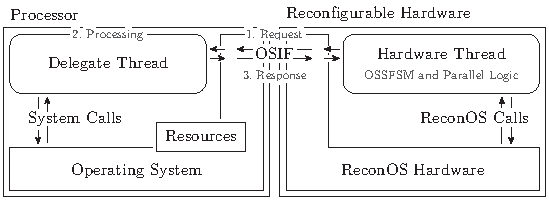
\includegraphics{../figures/delegate}
	\caption{ReconOS delegate mechanism in detail}
	\label{fig:delegate}
\end{figure}
 The \ac{OSIF} connects the hardware slot with the delegate thread as a
bidirectional \ac{FIFO} interface and allows message based communication. The
\acp{FIFO} are implemented in the reconfigurable fabric and attached to the
\ac{AXI} bus via an interface bridge. It provides access from the \ac{CPU} by
a set of memory mapped register and allows to read status bits or data words.
Furthermore, the \ac{OSIF} is attached to the interrupt input of the processor
to avoid busy waiting in the delegate threads, waiting for requests from the
hardware threads and consuming no processing time on the processor while being
blocked in a system call. The driver module provides blocking access to the
\ac{OSIF} by handling interrupts and accessing the memory mapped registers.

To illustrate the procedure of delegating an \ac{OS} call, figure
\ref{fig:delegate} sketches an exemplary \lstinline{MBOX_GET}. At first, the
hardware thread issues the request by writing the appropriate messages into
the \ac{OSIF}, namely an internal encoding of the command, followed by an
identification of the appropriate \ac{OS} resource and additional arguments.
The interrupt causes the delegate thread to wake up, read the messages from
the \ac{OSIF} and decode the commands. After executing the appropriate \ac{OS}
call, the delegate thread writes back an acknowledge into the \ac{OSIF} and,
optionally, the result of the system call. Following this process, the
exchange of a single message between two hardware threads via a mailbox
includes two interrupts implying context switches into the kernel space, the
handling of the mailbox by the kernel and the access of the \ac{OSIF} itself.
All these operations introduce a significant delay of thousands of clock
cycles and burden the processor with additional tasks. Furthermore, since the
benefits of a custom hardware implementation originate from its highly
parallel structures, the sequential execution enforced by the communication
via the central processor results in a bottleneck, limiting the full potential
of all hardware threads.

Besides the communication via system calls and synchronization primitives
handled by the delegate mechanism, the threads can also exchange data via the
shared memory interface. It provides access to the main memory but introduces
the same bottleneck of enforcing access in a sequential manner. Again, the
benefits of parallel execution are narrowed and performance is decreased. In
particular, streaming-like applications passing data from one thread to
another cannot be modeled efficiently by applying a shared memory model.
Instead, a method of exchanging data directly from one thread to another is
required.

\section{Interconnect Architecture}

Introducing a method of communication for hardware threads without involving
the processor includes several challenges. The delegate mechanism provides
complete transparency regarding the implementation mode of a thread and a
unified programming interface of communication primitives for both hardware
and software implementations. An interconnect implemented in the fabric of the
\ac{FPGA} must be integrated into the existing system transparently, allowing
all required communication by utilizing only limited resources and providing a
suitable programming model.

Besides ReconOS, there exist other operating systems leveraging the
multithreaded programming model and providing a transparent interface. The
most important and comparable framework is the hthreads project, focusing on
low-jitter hardware implementations of \ac{OS} functions \citep{AHK14}. It
provides similar functionality but follows a different approach as illustrated
by the block diagram in figure \ref{fig:hthreads}.
\begin{figure}[tb]
	\centering
	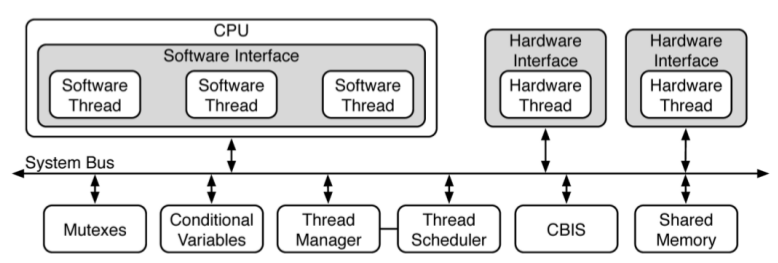
\includegraphics[width=10cm]{../figures/hthreads}
	\caption{Hthreads system block diagram \citep{ASA08}}
	\label{fig:hthreads}
\end{figure}
Instead of utilizing an existing \ac{OS} and its functions through a delegate
mechanism, it implements all resources together with scheduling and management
components in the reconfigurable fabric \citep{ASA08}. While this guarantees a
low-latency access to all components, the central system bus limits the
overall performance in high-load situation and the architecture is rather
unportable to standard \ac{OS} kernels or other platforms. However,
implementing  \ac{OS} functions on the \ac{FPGA} seems to be the best approach
to utilize the full potential of a hardware design in a hybrid multi-core
system. Adopting this idea for the ReconOS framework promises significant
speedups for many applications and seems to be crucial to utilize ReconOS in
modern \ac{PAC} designs.

Besides the implementation of \ac{OS} functions in hardware, both software and
hardware threads must be able to access these functions transparently through
a central interconnect. While hthreads utilizes a central bus for this task, a
bus structure, again, limits parallel access and performance. Choosing an
appropriate interconnect, just like the implementation mode of the resources,
seems to be a crucial step, highly dependent on the application and its
structure. Furthermore, since the system might be able to adapt itself to
upcoming requirements during runtime, the needs for the interconnect
structure might change after design time. Consequently, an interconnect
architecture should provide a flexible way of utilizing different structures
specified at design time and, additionally, allow a reconfiguration at run
time.

Figure \ref{fig:interconnect} illustrates the reconfigurable interconnect
architecture developed and presented in this thesis.
\begin{figure}[tb]
	\centering
	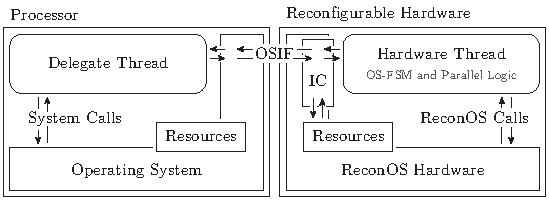
\includegraphics{../figures/interconnect}
	\caption{Reconfigurable interconnect}
	\label{fig:interconnect}
\end{figure}
It seamlessly integrates into the existing ReconOS architecture by utilizing
the existing interfaces. Instead of connecting the \ac{FIFO} based \acp{OSIF}
directly to the processor, the interconnect allows requests to be rerouted to
resources implemented on the \ac{FPGA}, by introducing a simple addressing
scheme together with a protocol described later. The hardware resources are
also connected to the interconnect via a \ac{FIFO} based interface and
communicate via messages to the different threads. To provide transparent
access to them, the idea of a delegate thread is adopted for software threads,
allowing them to interface with the system the same way a hardware threads
does. While the interconnect presents a fixed interface to the outside world,
its internal structure is hidden completely. This allows to implement
different structures, for example buses, rings, or crossbar interconnects, and
also allows internal reconfiguration at runtime without effecting the
connected components.

The following subsections describe the interconnect in detail and illustrate
its principles. Starting with an introduction of the interconnect interface
and the extended \ac{OSIF} protocol including its consequences for the
software implementation, the software delegate mechanism is explained and to
what extend it allows transparent access to the hardware resources. Finally,
the integration into the existing ReconOS toolchain will be considered.

\subsection{Interconnect Protocol}
The interconnect routes \ac{OSIF} messages between the different components,
mainly resources, hardware-, software-, and delegate threads. While the
original \ac{OSIF} was intended to be a point-to-point connection between the
hardware and its associated delegate thread, an addressing scheme was not
necessary and, additionally, the length of messages were defined implicitly by
its commands. For an interconnect routing messages to different destinations,
a more advanced protocol is required. Besides, at least, a destination
address, the interconnect also requires knowledge of the length of a message.
Figure \ref{fig:proto} shows the structure of a control word introduced for
the interconnect and send before the start of a message. To minimize the
changes of the hardware thread interface, they are not indicated by a separate
control flag.
\begin{figure}[tb]
	\centering
	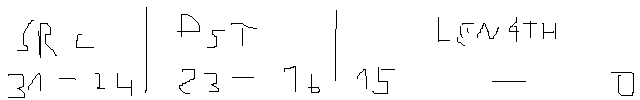
\includegraphics{../figures/proto}
	\caption{Control message preceding each message}
	\label{fig:proto}
\end{figure}
They consists out of a source and destination, as well as a length field,
indicating the number of following words. Since the address fields have a
length of eight bits, the number of addressable components is limited to 255,
which seems to be sufficient for typical applications. Anyway, the number of
threads and resources is limited by the available resources on the
\ac{FPGA}, as well as routing restrictions. The 16 bit wide length field
allows messages with a maximum number of 65,535 words, which, again, seems to
be sufficient for typical applications. However, it does not allow an endless
streaming of data, which must be split up into messages of fixed size.

Based on the control words, the internal interconnect structure is responsible
for routing the messages to the right destinations. Therefore, it must respect
the system's configuration, for example which resources are implemented in
hard- or software and which threads are currently running. It might allow
routing of messages between threads and resources, but also between threads
for direct communication. Generally, the software interface should always act
as a fallback and, therefore, be able to address all resources of the system.

For the hardware thread interface, the addressing scheme implies only marginal
changes. The \ac{OSIF} protocol itself remains unchanged, but is preceded by
the additional control word. However, it should be stated, how the control
world is composed for the different \ac{OSIF} calls. The length of a request
is set according to the command and, thereby, known implicitly. Although a
regular request should be routed to the delegate thread, the request itself
must be addressed to the targeted resource. This allows to transparently route
the request not to the delegate thread, but to a resource implemented in
hardware. Addressing such a request with the address of a delegate thread
would prevent such a transparent rerouting. To send back an acknowledge as
response to the hardware thread's request, the receiver must know the source
address, the request is originating from. Therefore, a hardware thread needs
to specify its own id as the source of the request. However, a thread does not
know its own id implicitly, since it depends on the execution mode and
scheduled slot determined at runtime. Consequently, an appropriate mechanism
is needed, allowing a thread to receive its runtime id. Querying the id
through a traditional \ac{OSIF} command is not possible, since the request
itself would require an id. Therefore, the ReconOS runtime sends, initially
on thread creation, the runtime id to the thread, which is responsible for
storing it.

\subsection{Interconnect Interface}
While the internal structure of the interconnect can be arbitrarily defined,
its external interface presented to the different ReconOS components is fixed.
This allows to develop a range of interconnect structures for different
requiremens of the applications. Furthermore, considering self-adaptive
features of the application and partial reconfiguration capabilities of the
\ac{FPGA}, the fixed external interface allows reconfiguration of the
interconnect during runtime. Figure \ref{fig:interconnect_if} presents the
interface, consisiting out of bidirectional \ac{FIFO} ports for each connected
component, namely the hardware threads, the hardware resources and the
processor.
\begin{figure}[tb]
	\centering
	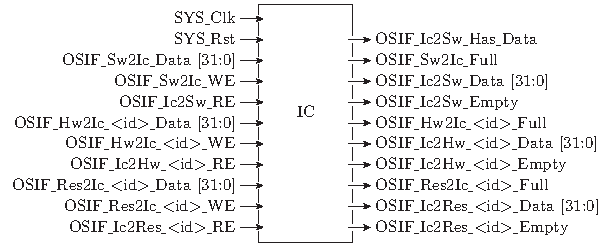
\includegraphics[width=12cm]{../figures/interconnect_if}
	\caption{Interface of reconfigurable interconnect}
	\label{fig:interconnect_if}
\end{figure}
Obviously, the interface depends on the number of hardware resources and
hardware threads and is generated accordingly. Therefore, an implemented
interconnect structure must also respect the variying number of ports. Note,
that all \ac{FIFO} interfaces are implemented as target ports, i.e. the
components connect their master or slave interfaces directly to the
interconnect, without a dedicated \ac{FIFO} core in between. This leaves the
decision where and when to buffer words to the interconnect, allowing more
flexible and optimized structures. For example, the interconnect might be
implemented using asynchronous multiplexers without the overhead of a
dedicated buffering \ac{FIFO}.

Introducing an addressing scheme with source and destination addresses, as
discussed in the previous section, allows to simplify the interface to the
processor. Originally, each of the \acp{OSIF} were attached individually
through a set of memory mapped registers to the processor. However, since the
kernel driver and system bus support only sequential access, the parallel
mapping could not be utilized for parallel access and provides no performance
benefits. Therefore, the interconnect provides a single \ac{FIFO} interface to
the processor and is responsible to arbitrate the different requests from the
hardware components. In software, the driver module provides an interface to
wait for and receive messages based on a filter, specifying a mask
(\lstinline{MASK}) and a reference value (\lstinline{BITS}). Whenever the
driver module reads a message, it routes it to the appropriate user-space
process satisfying \lstinline{CTRL & MASK == BITS}. To specify the filter, a
process issues the \lstinline{RECONOS_OSIF_SET_MASK} and
\lstinline{RECONOS_OSIF_SET_BITS} system calls after opening the appropriate
device file. For example, a delegate thread associated to slot 1 needs to
receive all messages originating from the associated hardware thread and
specifies a mask of \lstinline{0xFF000000}, together with a reference value of
\lstinline{0x01000000}. It only filters the source address, since the
destination address does not represent the delegate thread, but a specific
resource.

\subsection{Software Delegate Mechanism}

While hardware threads have direct access to the hardware resources, they use
a delegate mechanism to access resources implemented in software. Adopting
this approach for software threads, which have direct access to resources
managed on the processor but no access to the resources in hardware, enables
them a transparent access to all resources, independent from their
implementation mode. However, software threads are much more flexible in terms
of instances and termination, and a fixed concept of slots for software
threads would be unsuitable. Furthermore, additional hardware for each
software thread is not desirable. Since the processor itself is connected to
the interconnect via the single \ac{OSIF} interface, the software application
is able to send messages in the same way a hardware thread does. A resource
utilizing delegate thread with a dedicated interface becomes unnecessary and
all software threads can share the same \ac{OSIF} arbitrated by the driver
module.

Utilizing the \ac{OSIF} interface enables software threads to access hardware
resources, but provide no transparent abstraction. To hide the underlying
implementation of a resource request from the software thread, the runtime
needs to know the implementation mode of each resource, enabling it to execute
the appropriate system call or interface with the hardware. Since every
resource is represented by a data structure during runtime, it can be easily
extended by a flag indicating the implementation mode. Listing
\ref{lst:mbox_get} illustrates the concept by presenting a part of the
\lstinline{mbox_get} implementation.
\begin{lstlisting}[
	language=C,
	caption={Excerp from the \lstinline{mbox_get} implementation},
	label={lst:mbox_get},
	float=tb
]
if (res->mode == RECONOS_RESOURCE_MODE_SW) {
	return mbox_get(res->ptr);
} else if (res->mode == RECONOS_RESOURCE_MODE_HW) {
	msg[0] = (run_id << 24) | (res->id << 16) | 0x00000001;
	msg[1] = OSIF_CMD_MBOX_GET;
	reconos_thread_swslot_write(rt, msg, 2);
	reconos_thread_swslot_read(rt, msg, 2);
	return msg[1];
}
\end{lstlisting}
Originally, the software threads directly issue the system call as in line 2.
To hide the different implementation modes, ReconOS provides an abstraction
for each operation. Based on the current mode of the resource determined
during runtime, it either issues a regular system call (line 2) or sends a
request to the hardware resource (line 4-6), followed by a wait for the
response (line 8). Note, that the threads send requests as described in the
previous section, including control word with a thread id \lstinline{run_id}
determined at runtime. The driver handles the underlying access to the
\ac{OSIF}, arbitrates parallel request and routes the response back to the
appropriate thread.

Introducing an abstraction for all resource operations also provides a unified
interface for all implementation modes of a thread. Independently from the
language used to implement a ReconOS thread, the same \ac{API} can be
utilized. For example, originally, the \ac{VHDL} implementation called
\lstinline{osif_mbox_get}, while the software directly called
\lstinline{mbox_get}. Together with the support for \ac{HLS}, all thread
descriptions are now able to perform the operation by calling
\lstinline{MBOX_GET} together with an automatically generated identifier
available in all descriptions.

\subsection{Hardware resources}
As already covered in the protocol section, a request to a resource, either
handled via a delegate thread in software or directly in hardware, consists
out of the control word, followed by the original \ac{OSIF} command, i.e. the
encoding of the command, followed by additional arguments. While the delegate
thread translate the encoding into the appropriate system call executed by the
operating system, a hardware resource must implement all logic independently
of any \ac{OS} features. Thereby, since many system calls are performed in a
blocking manner, the implementations of the resources incorporate scheduling
components circumventing the scheduling of the operating system. Since the
resources have no access to any scheduling components, they can only implement
basic algorithms, for example \acl{FIFO}. However, for hardware threads,
scheduling has only limited influence, since all threads can be executed in
parallel. Since hardware resources are mainly targeting hardware to hardware
communication, the limited scheduling capabilities are acceptable.

Considering self-adapting systems with changing execution modes of threads
suggests to reconfigure the mode of a resource analogously. For example, if
threads are migrated from hardware to software, it might be reasonable to also
migrate an appropriate resource used by the threads. While the infrastructure
itself is designed in a flexible way and could support such migrations, it
includes similar challenges as arising from thread migration. Although this
self-adaptiveness constitutes a relevant research topic, it is not targeted in
this thesis, assuming a fixed configuration of resources, specified at design
time.

\subsection{Toolchain Integration}
To make hardware resources available to the developer, the toolchain must
provide a way to specify the implementation mode of a resource and handle the
generation of an appropriate interconnect. Listing \ref{lst:hwres_cfg} shows
an example of two mailboxes, one implemented in software, the other one
implemented in hardware.
\begin{lstlisting}[
	caption={Excerp from the ReconOS configuration},
	label={lst:hwres_cfg},
	float=tb
]
[ResourceGroup@Eval]
MboxSw = sw,mbox,2
MboxHw = hw,mbox,2
\end{lstlisting}
As the listing indicates, changing the implementation mode of a resource can
be achieved by adding a flag to the configuration file and, therefore, is
totally transparent to the developer.

Additionally to the manual specification of implementation modes, the
toolchain could implement algorithms to determine automatically the best
implementation mode. For example, by considering the implementation modes of
threads using a specific resource, an optimized mode could be determined.
However, when considering self-adapting systems reconfiguring the execution
modes of threads at runtime, the toolchain cannot decide on an optimal
solution.

\section{Evaluation}
To prove the feasibility of the proposed interconnect design and illustrate
the benefits of a direct hardware communication, an extensive evaluation is
presented in this section. The interconnect details discussed so far
emphasized only the external interface and disregarded its internal structure.
However, for an evaluation of the system an actual implementation is required.
Therefore, a crossbar based interconnect consisting of routing and arbitration
components will be presented. Based on this interconnect, two different
hardware resources are evaluated in a prototypical application and compared to
the original design. All evaluation is performed using the ZedBoard, featuring
a Zynq XC7Z020-CLG484.

\subsection{Crossbar Interconnect}
The interconnect specifies only the external interface and functionality, but
not its internal implementation. This allows to realize different
architectures, ranging from bus structures to ring based protocols. Obviously,
every structure provides unique benefits and drawbacks in terms of
performance, parallelism or resource utilization, making the choice highly
depended on the application's demands. For this evaluation, a high-performance
crossbar interconnect was implemented, providing parallelism and short delays
at a cost of a higher resource utilization.

Figure \ref{fig:crossbar} shows the structure of the crossbar interconnect,
consisting out of arbitration and routing components, as well as \ac{FIFO}
buffers. Note, that the number of ports depends on the number of threads and
resources and are generated accordingly during implementation.
\begin{figure}[tb]
	\centering
	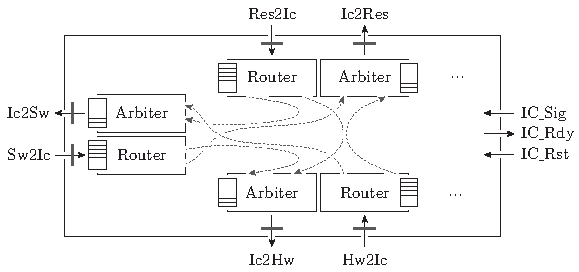
\includegraphics{../figures/crossbar}
	\caption{Crossbar interconnect}
	\label{fig:crossbar}
\end{figure}
The procedure of routing a message from a master port to the appropriate
output slave includes three major steps. At first, the sending component
writes its data to the associated master port, connected to a buffering
\ac{FIFO} temporarily storing the message data. Whenever this data is
available at the slave port connected to the routing component, it reads the
control word and routes the entire message to the destination arbiter. Since
no delay introducing buffering is present in between the routing and
arbitration components, the term routing might be misleading. Rather writing
messages, the router asynchronously multiplexes the slave interface of the
incoming \ac{FIFO} the the appropriate output ports. Similarly, the
arbitration components demultiplexes all incoming ports to the outgoing
buffering \ac{FIFO}. Since the internal connections between routing and
arbitration components are asynchronous, the external ports are buffered by
additional \acp{FIFO}. While the incoming buffers are essential, the outgoing
ones could be omitted. However, as it turned out during the implementation of
different slave components connecting the interconnect signals asynchronously,
timing becomes a heavily limiting factor and even a small interconnect does
not meet the required timing constraints. Therefore, the outgoing buffers
shorten the critical path significantly and eliminating timing issues.

\subsubsection{Routing Component}
As illustrated in figure \ref{fig:crossbar}, the routing component multiplexes
the single slave input to multiple output ports based on the control word.
Therefore, it implements an asynchronous multiplexer controlled by a bit
vector indicating the targeted output port and controlled by a state machine
as illustrated in figure \ref{fig:router_fsm}.
\begin{figure}[tb]
	\centering
	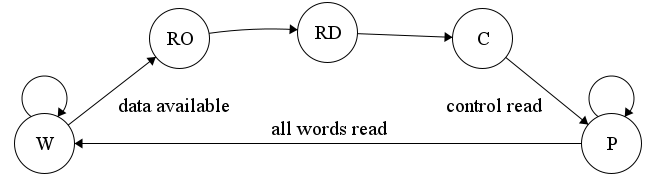
\includegraphics{../figures/router_fsm}
	\caption{\acs{FSM} of router}
	\label{fig:router_fsm}
\end{figure}
In its initial state \emph{W} the router waits for a message becoming
available at the incoming slave port and reads the first control word. States
\emph{RO} and \emph{RD} then perform the routing by considering the
destination address of the message and setting the appropriate select bit for
the multiplexer. While \emph{RO} compares the destination address to the known
ids of the output ports, \emph{RD} represent the default routing target. After
determining the destination port for the message, the control word is written
to the output in state \emph{C}, followed by the payload data in state
\emph{P}. After the entire message is transferred, the router returns to its
initial state \emph{W} and waits for the next message.

Considering this procedure, it takes only three clock cycles until the first
word of the message is present at the output port. Assuming, that all messages
can be handled by \emph{RO}, the state \emph{RD} can be eliminated, resulting
in a delay of two clock cycles.

\subsubsection{Arbitration Component}
While the router multiplexes a single input \ac{FIFO} to the appropriate
output port, the arbiter demultiplexes multiple inputs to a single output
\ac{FIFO}. Therefore, it implements a round-robin scheduler, processing the
incoming messages one after another. Note, that the implemented scheduler does
not cycle through all inputs sequentially, i.e. a single request is processed
immediately without a delay proportional to the number of input ports. Again,
a bit vector is used as a selection for the demultiplexer and controlled by
the state machine implementing the round-robin algorithm as illustrated in
figure \ref{fig:arbiter_fsm}.
\begin{figure}[tb]
	\centering
	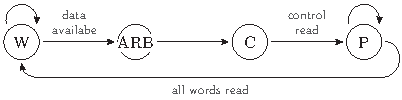
\includegraphics{../figures/arbiter_fsm}
	\caption{\acs{FSM} of arbiter}
	\label{fig:arbiter_fsm}
\end{figure}
Initially in state \emph{W}, the arbiter waits for a message being present at
one of the input \acp{FIFO}. Whenever data is available, it processes the
request in a round-robin fashion in state \emph{ARB}, by determining the
\ac{LSB} of the input requests by
\lstinline{req and std_logic_vector(unsigned(not(req)) + 1)} and masking it
out for the next turn. This procedure introduces no delay for single request
compared to an iterative approach looping through the inputs. After
determining the next message to arbitrate, the control word is written to the
output in state \emph{C}, followed by the rest of the message's data in state
\emph{P}. When all words are read, the arbiter return to state \emph{W} and
processes the next message.

\subsubsection{Resource Utilization}
While the crossbar interconnect allows parallel transaction between different
ports and a low delay of a few clock cycles, it consumes a relatively high
amount of resources. As stated, the interconnect mainly consists out of the
routing and arbitration components. Figure \ref{fig:crossbar_util} shows their
resource utilization, increasing with the number of ports.
\begin{figure}
	\centering
	\begin{subfigure}{0.49\textwidth}
		\centering
		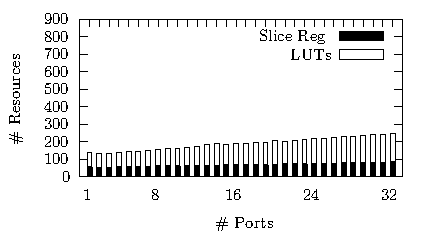
\includegraphics[width=\textwidth]{../figures/eval_router}
		\caption{Routing component}
		\label{fig:crossbar_util_router}
	\end{subfigure}
	\begin{subfigure}{0.49\textwidth}
		\centering
		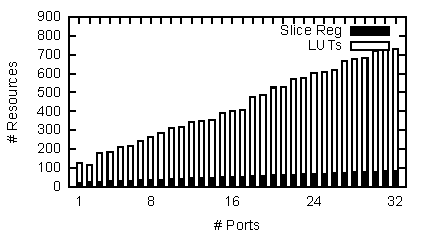
\includegraphics[width=\textwidth]{../figures/eval_arbiter}
		\caption{Arbitration component}
		\label{fig:crossbar_util_arbiter}
	\end{subfigure}
	\caption{Resource utilization for different number of ports}
	\label{fig:crossbar_util}
\end{figure}
Thereby, the number of \acp{LUT} shows a stronger growth than the number of
registers, since most of the resources are consumed by the combination
multiplexers, heavily influenced by the number of ports. Furthermore, the
arbiter's multiplexers need significantly more resources compared to the
router's counterparts, since they multiplex the 32-bit wide data ports, while
the router connects the incoming data port directly to all outgoing ports.

In total, even a rather unrealistic high number of ports results in an
acceptable resource utilization without timing issues caused by the
interconnect.

%Additionally to the routing and arbitration components, the entire
%interconnect also includes several \acp{FIFO} for buffering of the external
%interfaces. Table \ref{tab:crossbar_util} shows the resource utilization for
%an entire interconnect for a single hardware resource and three hardware
%threads.
%+---------------------------------------------------------------+
%| Module      | Slices* | Slice Reg | LUTs | LUTRAM | BRAM/FIFO |
%+---------------------------------------------------------------+
%| FIFOs       | 124     | 65        | 358  | 240    | 0         |
%| Routing     | 212     | 266       | 359  | 0      | 0         |
%| Arbitration | 167     | 114       | 452  | 0      | 0         |
%+---------------------------------------------------------------+
%| Total       | 503     | 445       | 1169 | 240    | 0         |
%+---------------------------------------------------------------+
%\begin{table}
%	\centering
%	\captionabove{Resource utilization of crossbar interconnect}
%	\label{tab:crossbar_util}
%	\begin{tabular}{lcccc}
%	\hline
%	\textbf{Type} & \textbf{Slices} & \textbf{Slice Reg} & \textbf{LUTs} & \textbf{LUTRAM}\\
%	\hline
%	\acp{FIFO} & 124 (24.7\%) & 65 (14.6\%) & 358 (30.6\%) & 240 (100.0\%)\\
%	Routing & 212 (42,1\%) & 266 (59.8\%) & 359 (30.7\%) & 0 (0.0\%)\\
%	Arbitration & 167 (30.2\%) & 114 (25.6\%) & 452 (38.7\%) & 0 (0.0\%)\\
%	\hline
%	Total & 503 (100.0\%) & 445 (100.0\%) & 1169 (100.0\%) & 240 (100.0\%)\\
%	\hline
%	\end{tabular}
%\end{table}

%+------+---------+---------+-----------+-----------+
%| #Res | Module  | Slices* | Slice Reg | LUTs      |
%+------+---------+---------+-----------+-----------+
%| 1    | arbiter | 31      | 56        | 82        |
%| 1    | router  | 17      | 22        | 102       |
%| 2    | arbiter | 45      | 54        | 77        |
%| 2    | router  | 21      | 24        | 92        |
%| 3    | arbiter | 51      | 55        | 81        |
%| 3    | router  | 63      | 26        | 152       |
%| 4    | arbiter | 46      | 56        | 82        |
%| 4    | router  | 61      | 28        | 156       |
%| 5    | arbiter | 50      | 57        | 85        |
%| 5    | router  | 48      | 30        | 180       |
%| 6    | arbiter | 55      | 59        | 91        |
%| 6    | router  | 55      | 34        | 206       |
%| 7    | arbiter | 55      | 59        | 91        |
%| 7    | router  | 55      | 34        | 206       |
%| 8    | arbiter | 52      | 62        | 93        |
%| 8    | router  | 64      | 36        | 229       |
%+------+---------+---------+-----------+-----------+


\subsection{Propagation Time}
To evaluate the performance of a hardware resource compared to its
implementation in software, the commonly used mailbox was chosen as a
representative synchronization object. The following subsections present a
short explanation of the hardware implementation using \ac{HLS}, followed by
an evaluation of several turnaround times.
\subsubsection{Mailbox}
A mailbox constitute a basic synchronization primitive allowing to exchange
single data words by providing thread safe put and get methods. In software,
the mailbox is implemented as a memory area with protected access through a
semaphore, counting the number of available words and handling blocking calls.
Figure \ref{fig:mbox_hw_struct} presents an equivalent hardware
implementation, utilizing multiple \ac{FIFO} buffers for data words and
pending requests.
\begin{figure}
	\centering
	\begin{subfigure}{0.49\textwidth}
		\centering
		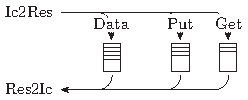
\includegraphics{../figures/mbox_hw_struct}
		\caption{Overall structure}
		\label{fig:mbox_hw_struct}
	\end{subfigure}
	\begin{subfigure}{0.49\textwidth}
		\centering
		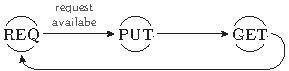
\includegraphics{../figures/mbox_hw_fsm}
		\caption{Control logic}
		\label{fig:mbox_hw_fsm}
	\end{subfigure}
	\caption{Mailbox implementation in hardware}
	\label{fig:mbox_hw}
\end{figure}
Each request is enqueued into the corresponding \ac{FIFO} to free the input
\ac{FIFO} in case of a blocking call, for example an \lstinline{mbox_get} on
an empty mailbox. Besides the request \acp{FIFO}, a single data buffer models
the memory area used in software, to store the putted data words until the
next get request. Access to the different \acp{FIFO} is handled by a state
machine as illustrated in figure \ref{fig:mbox_hw_fsm}. The state machine
cycles between three main states \emph{REQ}, \emph{PUT} and \emph{GET},
consisting out of multiple sub-states. \emph{REQ} handles the incoming request
from the hardware threads, decodes them and enqueues them into the appropriate
request buffers. Afterwards, \emph{PUT} and \emph{GET} check the queues for
pending requests and process them. While put requests store the transmitted
data words in the data buffer, get requests read out the stored words and
sends them back to the issuing threads. Therefore, the request buffers,
additionally, store the thread ids for each request.

While implementing this structure using Vivado HLS simplified the handling of
\ac{FIFO} buffers dramatically, it also pointed out the limitations of the C
language to model parallel structures. Since the \emph{REQ} state only writes
to the request \acp{FIFO} and the \emph{PUT} and \emph{GET} states only read
from them, both could be implemented in parallel and independently from each
other. However, C does not allow to specify concurrent blocks.

\subsubsection{Results}
To measure the performance of the mailbox, table \ref{tab:mbox_turn} shows the
turnaround times for combinations of different resource implementations,
thread execution modes and processor loads averaged over 10000 measurements.
The turnaround time represents the period between the execution of the put
operation and the return of get operation. The destination thread performs an
\lstinline{MBOX_GET} and, since the targeted mailbox is empty, blocks in this
call. After that, the source thread performs an \lstinline{MBOX_PUT} and, in
consequence, the blocking get operation of the destination thread returns.
Before the put operation and after the return of the get operation, both
threads save a time stamp, used to calculate the turnaround time as its
difference. Since an application typically puts some load on the processor,
the measurements were performed for both low and high system loads. While for
low load situations only the evaluation threads were executed, processor load
was created for the high load measurements by soft- and hardware worker
threads, executing arbitrary operations and communicating frequently. To
eliminate uncertainty, the measurements were performed on a single processor
system, disabling the second core using the kernel parameter
\lstinline{maxcpus=1}.

\begin{table}
	\scriptsize
	\centering
	\captionabove{Turnaround times for mailbox in clock cycles of $\SI{100}{\mega\hertz}$}
	\label{tab:mbox_turn}
	\begin{tabular}{llcccc}
	\hline
	\textbf{Mode} & \textbf{Load} & \textbf{Hw-Sw} & \textbf{Hw-Hw} & \textbf{Sw-Sw} & \textbf{Sw-Hw}\\
	\hline
	Hardware & Low & 3311 & 33 & 2485 & 301\\
	Hardware & High & 3912 & 33 & 2730 & 286\\
	Software & Low & 4093 & 3821 & 1094 & 1710\\
	Software & High & 4769 & 4591 & 1364 & 1935\\
	\hline
	\end{tabular}
\end{table}
As table \ref{tab:mbox_turn} indicates, a mailbox implemented in hardware
provides a significant speedup for hardware to hardware communication.
Furthermore, the communication is performed offside the processor and,
therefore, not influenced by the system's load and free of any jitter. Besides
the expected speedup for hardware to hardware communication, a hardware
resources also provides significant speedup for software to hardware
communication. While for a software resource the delegate blocks in the
appropriate system call and needs to be scheduled to send the result to the
hardware thread, the hardware resource is directly interfaced by the source
thread, avoiding an additional thread switch. The same reason applies for the
hardware to software processing, since no thread switch from the delegate to
the user thread is necessary.

Alltogether, a hardware resources outperforms its software counterpart in
every case a hardware thread is involved. However, it circumvents the
scheduling of software threads by the operating system, which should be
considered when selecting the implementation mode. Furhtermode, additional
hardware resources are required and many hardware resources may lead to timing
issues.

\subsection{Image Streaming}
While the synchronization of hardware threads benefits significantly from an
implementation of resources in hardware, data exchange is still limited by the
performance of the shared memory interface. The currently implemented
communication primitives does not provide an abstraction for data streaming
from one thread to another. Even though the memory interface provides fast
access to the main memory, it does not support parallel access for multiple
threads. Instead, all requests are serialized and processed sequentially. For
multiple threads exchanging data concurrently, this enforced sentimentality
limits the performance and puts significant load on the memory interface.

The following sections introduce the pipe as a new abstraction for streaming
data and evaluate it by means of an image processing application, applying
line based filters in multiple threads.

\subsubsection{Pipe}
The pipe originates from the field of inter-process communication and provides
a \ac{FIFO} based interface for exchanging data. It seems to be suitable to
abstract a unidirectional stream between different threads. While traditional
pipes in software provide a buffer storing the written data until it is read,
restricted on-chip memory on the \ac{FPGA} limits buffering for a hardware
implementation. Therefore, the ReconOS pipe implementation does not utilize a
dedicated buffer but directly forwards the data to the destination thread. The
write method blocks until a corresponding read method is called and writes
directly to the destination buffer. Analogously, the read method blocks until
a write request occurs and finishes. Note, that a pipe represents a direct
connection between two threads and does not provide any support for
concurrently occurring reads or writes on the same pipe. This must be handled
by the developer by introducing appropriate synchronization mechanisms,
serializing access and preventing concurrent requests.

Table \ref{tab:pipe_api} show the \ac{API} of the ReconOS pipe for C,
\ac{VHDL} and \ac{HLS} implementations of threads.
\begin{table}
	\scriptsize
	\centering
	\captionabove{\acs{API} of the ReconOS pipe}
	\label{tab:pipe_api}
	\begin{tabular}{ll}
	\hline
	\textbf{Command} & \textbf{Function (C, \acs{VHDL}, \acs{HLS})}\\
	\hline
	Write & \lstinline{int PIPE_WRITE(res, buf, len)}\\
	& \lstinline{PIPE_WRITE(i_osif, o_osif, i_ram, o_ram, res, len, lenrt)}\\
	& \lstinline{int PIPE_WRITE(res, buf, len)}\\
	\hline
	Read & \lstinline{int PIPE_READ(res, buf, len)}\\
	& \lstinline{PIPE_READ(i_osif, o_osif, i_ram, o_ram, res, len, lenrt)}\\
	& \lstinline{int PIPE_READ(res, buf, len)}\\
	\hline
	\end{tabular}
\end{table}
In the function definitions illustrated as pseudo-code, \lstinline{res}
represents the resource handle generated automatically during the build
process, \lstinline{buf} points to a data buffer and \lstinline{len} indicates
the number of bytes to read or write. Both functions return the number of
handled bytes, which might differ from the requested length. In that case, the
caller is responsible to handle missing data. Note, that the \ac{HLS} and C
functions have the same signature, allowing to compile an \ac{HLS} description
without modifications for software execution. The \ac{VHDL} function,
additionally, include the \lstinline{i_osif}, \lstinline{o_osif},
\lstinline{i_ram} and \lstinline{o_ram} records and provide the
\lstinline{lenrt} output signal instead of a return value. To illustrate the
usage of the pipe implementation, listing \ref{lst:pipe_exmpl} show an
exemplary hardware thread written in Vivado HLS, reading data from the main
memory and writing it to an outgoing pipe.
\begin{lstlisting}[
	language=C,
	caption={Exemplary hardware thread using the ReconOS pipe},
	label={lst:pipe_exmpl},
	float=tb
]
THREAD_ENTRY() {
	THREAD_INIT();
	RAM(uint32, 128, line);

	uint32 addr = MBOX_GET(read_cmd);

	MEM_READ(addr, line, 512);
	PIPE_WRITE(s0_out, line, 512);
}
\end{lstlisting}
Therefore, it receives an address via a mailbox, reads a specified number of
bytes from that address to a local ram and writes the data to the pipe
\lstinline{s0_out}.

In software the ReconOS pipe is implemented by, basically, two semaphores,
indicating read and write operations as sketched in listing \ref{lst:pipe_sw}.
\begin{lstlisting}[
	language=C,
	caption={Software implementation of ReconOS pipe},
	label={lst:pipe_sw},
	morekeywords={ssize_t},
	float=tb
]
ssize_t pipe_write(...) {
	sem_wait(&pipe->read);
	pipe->len = min(pipe->len, len);
	memcpy(pipe->buf, buf, pipe->len);
	sem_post(&pipe->write);
	return pipe->len;
}

ssize_t pipe_read(...) {
	pipe->len = len;
	pipe->buf = buf;
	sem_post(&pipe->read);
	sem_wait(&pipe->write);
	return pipe->len;
}
\end{lstlisting}
Reading from the pipe stores a pointer to the destination buffer in an
internal data structure, posts the read semaphore and waits for the write
semaphore. In contrast, the write waits for the read semaphore, copies the
data from the source to the destination buffer and posts the write semaphore.

For its hardware implementation, the ReconOS pipe specifies an appropriate
\ac{OSIF} protocol as illustrated in figure \ref{fig:pipe_hw_osif}.
\begin{figure}
	\centering
	\begin{subfigure}{0.49\textwidth}
		\centering
		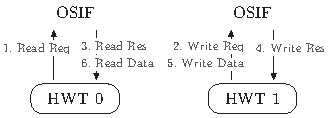
\includegraphics{../figures/pipe_osif}
		\caption{\acs{OSIF} protocol}
		\label{fig:pipe_hw_osif}
	\end{subfigure}
	\begin{subfigure}{0.49\textwidth}
		\centering
		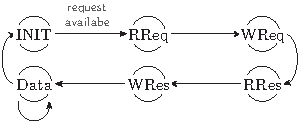
\includegraphics{../figures/pipe_fsm}
		\caption{Control logic}
		\label{fig:pipe_hw_fsm}
	\end{subfigure}
	\caption{Hardware implementation of ReconOS pipe}
	\label{fig:pipe_hw}
\end{figure}
For both writing and reading, the hardware thread sends an encoding of the
command, followed by the number of bytes to write or read, respectively. In
response to both requests, the pipe sends back an acknowledge to the threads,
indicating the number of actual bytes, i.e. the minimum of the read and write
request's lengths. Through that mechanism, the pipe mimics the blocking calls
to the semaphore in the software implementation. While the synchronization is
handled by the centralized resource, the data transfer could be processed via
direct thread interconnects. However, the data is transferred to the pipe
resource and then send back to the destination thread. While this design
introduces a delay of a few clock cycles, it eliminates the need for
additional interconnect links, resulting in lower resource utilization and
improved timing. Based on this protocol, figure \ref{fig:pipe_hw_fsm} shows
the appropriate control logic of the hardware implementation. In its states
\emph{INIT}, \emph{RReq} and \emph{WReq} it waits for a read and write
request. Thereby, the order in which the request arrive does not matter. After
both request are received, the pipe outputs the responses in states
\emph{RRes} and \emph{WRes}. Since the response to the reading thread must
arrive before the payload data, it is send before the write response. Finally,
in state \emph{Data} the resource forwards the data received from the writing
thread and returns to its initial state afterwards.

\subsubsection{Results}
Based on the pipe implementation, table \ref{tab:pipe_turn} shows, analogously
to the mailbox evaluation, the turnaround times for different thread
combinations and load situations. Measured by subtracting time stamps taken at
the start of the read command and after the completion of the write command, they represent the time needed for transferring a number of bytes from the source thread to the destination thread.
\begin{table}
	\scriptsize
	\centering
	\captionabove{Turnaround times for pipe with 512 bytes in clock cycles of $\SI{100}{\mega\hertz}$}
	\label{tab:pipe_turn}
	\begin{tabular}{llcccc}
	\hline
	\textbf{Mode} & \textbf{Load} & \textbf{Hw-Sw} & \textbf{Hw-Hw} & \textbf{Sw-Sw} & \textbf{Sw-Hw}\\
	\hline
	Hardware & Low & 7434 & 172 & 33701 & 5857\\
	Hardware & High & 8996 & 172 & 33524 & 5738\\
	Software & Low & 7620 & 13619 & 1242 & 7208\\
	Software & High & 9820 & 14339 & 1534 & 6744\\
	\hline
	\end{tabular}
\end{table}
The execution times in table \ref{tab:pipe_turn} result from transferring 512
bytes or 128 words respectively and are averaged over 10000 measurements. As
expected, the same relations as described for the mailbox can be applied,
certainly with even more significant differences, especially for communication
between threads of the same implementation mode. For example the hardware
implementation of a pipe compared to its handling via the delegate thread
provides a speedup of around 80 in case of communication between two hardware
threads. The discrepancy between the execution times of software communication
via a hardware resource and hardware communication via a software resource
results from additional thread scheduling and interrupt handling needed in the
latter case.

To demonstrate the benefits of a pipe implemented in hardware in a real world
example and to compare its performance to a classical shared memory approach,
an image processing application was implemented in various versions. It
consists out of multiple threads, applying line based modification to the
image and exchanging its lines in a pipeline as shown in figure
\ref{fig:img_proc}. It consist out of two filter threads, the first one
brightening up the image by multiplying each pixel with $1.2$ and the second
one mirroring the image horizontally. In both cases, the original and modified
images are read from and written to the shared memory to make them accessible
from the processor. Therefore, the read and write threads receive an address
via mailbox and the write thread sends an acknowledge back when finished
writing. Communication between the different filter threads is handled by a
pipe or shared memory in combination with mailboxes for synchronization.
\begin{figure}
	\centering
	%\begin{subfigure}{0.49\textwidth}
	%	\centering
	%	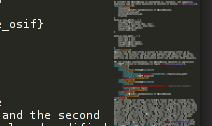
\includegraphics[width=0.97\textwidth]{../figures/img_proc_pipe}
	%	\caption{Pipe}
	%	\label{fig:img_proc_pipe}
	%\end{subfigure}
	%\begin{subfigure}{0.49\textwidth}
	%	\centering
	%	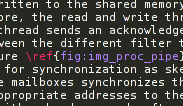
\includegraphics[width=0.97\textwidth]{../figures/img_proc_mem}
	%	\caption{Shared memory}
	%	\label{fig:img_proc_mem}
	%\end{subfigure}
	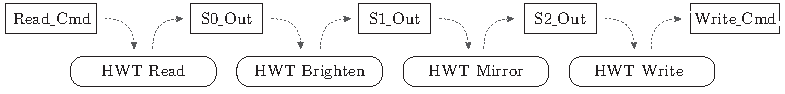
\includegraphics[width=0.97\textwidth]{../figures/img_proc}
	\caption{Image processing application}
	\label{fig:img_proc}
\end{figure}
The mailboxes synchronizes the access to the shared memory and propagate the
appropriate addresses to the next thread. Both versions were implemented with
a hardware and software implementation of the used resources, namely the pipe
and mailbox, and evaluated by measuring the processing time for a single image
of 128x205 pixels. They are measured by subtracting the time stamps captured
when sending the initial command to the read thread and after receiving the
acknowledge from the write thread. As the turnaround times already suggest,
the software implementation of the pipes leads to the slowest execution time
of $\SI{88.60}{\milli\second}$, followed by the software implementation of the
mboxes requiring $\SI{24.44}{\milli\second}$. The communication involving the
processor slows down the system dramatically, especially the transfer of data
via the \ac{OSIF} is significantly slower than via shared memory.
Consequently, the hardware implementations of the synchronization primitives
provide better results, namely $\SI{7.12}{\milli\second}$ for the classical
shared memory approach and $\SI{6.72}{\milli\second}$ for the pipe
implementation. While in the software case the communication overhead exceeds
the computation time, the hardware versions are limited by the processing time
of the image. This also explains the marginal difference between the pipe and
shared memory implementation, since during processing the memory interface is
free and both threads can share it efficiently.


\todo{conclusion?}